\documentclass[11pt, a4paper]{article} 
\usepackage{amssymb}
\usepackage[shortlabels]{enumitem}
\usepackage[fleqn]{amsmath} % fleqn: flush left equations <-- Left-flush equations
\usepackage{graphicx}
\usepackage{pgfplots}
\usepackage{hyperref, url}
\usepackage[margin=2cm, top=2cm]{geometry}
\graphicspath{{./img/}}
\newcommand\setItemNumber[1]{\setcounter{enumi}{\numexpr#1-1\relax}}
\newcommand*{\mybox}[1]{\framebox{#1}}
\newcommand{\tuple}[1]{$\langle #1 \rangle$} 
\newcommand{\stuple}[1]{$\langle$#1$\rangle$} % ordered pair with strings inside
\newcommand{\forceindent}{\leavevmode{\parindent=1em\indent}}

\title{\bf Homework 1\\[1ex]
\rm\normalsize CS250 Discrete Structures I, Winter 2020 }
\date{\normalsize Due: April 12, 2020}
\author{\normalsize Armant Touche}

\begin{document} 
\vspace{0cm}\maketitle 
	\section{Exercises} Chapter 1: Counting\newline
	\paragraph{Problem 1} 1.1 Additive and Multiplicative Principles (pages 67-69)\newline
	From section 1.1 in the textbook, complete exercises 4 and 10

    \begin{enumerate} 
    
        %4
        \setItemNumber{4}
        \item We usually write numbers in decimal form (or base 10), meaning numbers are composed using 10 different “digits” $\{0,1,...,9\}$. Sometimes though it is useful to write numbers hexadecimal or base 16. Now there are 16 distinct digits that can be used to form numbers: $\{0,1,...,9,A,B,C,D,E,F\}$. So for example, a 3 a 3 digit hexadecimal number might be 2B8.
        \begin{enumerate}[(a)]

            \item How many 2-digit hexadecimals are there in which the first digit is E or F? Explain your answer in terms of the additive principle (using either events or sets).
            
            There are sixteen 2-digit hexadecimal numbers that start with E and sixteen 2-digit hexadecimal. To answer the question, we use the additive principle because the event that a number start with either an E or F are independent of one another we simply add the two disjoint events together to get the total number of possible 2-digit hexadecimal numbers that either start with E or F. Resulting in thirty-two possible 2-digit hexadecimal numbers that start with either E or F.

            \item Explain why your answer to the previous part is correct in terms of the multiplicative principle (using either events or sets). Why do both the additive and multiplicative principles give you the same answer?

                if we were to use the multiplicative rule in the previous answer, I would say, let A be the event that a hexedecimal number is 2-digit starting digit is E or F. There are only two ways for that to happen. Let B be the number possible digits to follow which is sixteen. $A\cap B = 2 \cdot 16 = 32$. This result is the same answer from using the additive rule.
            
            \item How many 3-digit hexadecimals start with a letter (A-F) and end with a numeral (0-9)? Explain.

                There six number of possiblities for the first digit to be (A-F), sixteen possibilities for the second digit (0-F), and lastly, ten possiblities for the last digit (0-9). Multiplying $6 \cdot 16 \cdot 10 = 960$ number of possible 3-digit hexadecimal numbers that start with (A-F) and end with a numeral (0-9). 

            \item How many 3-digit hexadecimals start with a letter (A-F) or end with a numeral (0-9) (or both)? Explain.

                Since this event is considered a union and isn't exclusive of one another, meaning, that both can or cannot happen. Let A be the number of 3-digit hexadecimal that start with (A-F). I am going to use the multliplicative rule for $A$. $A = 6 \cdot 16 \cdot 16 = 1536$ possible 3-digit number that starts with (A-F). Let $B$ be the number of 3-digit numbers that end with (0-9). $B = 16 \cdot 16 \cdot 10 = 2560$ possible 3-digit numbers that end with (0-9). We are asked $A \cup B$ which is just $A + B - (A \cap B)$. The less portion $(A \cap B)$ is meant to account for not double counting since these events can happen at the sametime. The answer for $A \cup B = A + B - (A\cap B) = 1536 + 2560 - 960 = 3136$ possible 3-digit numbers that either start with (A-F) or end with (0-9) or both.
        

        \end{enumerate}

        %10
        \setItemNumber{10}
        \item How many positive integers less than 1000 are multiples of 3, 5, or 7? Explain your answer using the Principle of Inclusion/Exclusion.

            Let $A$ be the number of multiples in 1000 that have a common factor of 3, $B$ be the number of multiples in 1000 that have a common factor of 5, and $C$ be the number of multiples in 100 that have a common factor of 7. $A = \lfloor 1000 \div 3 \rfloor = 333$, $B = \lfloor 1000 \div 5 \rfloor = 200$, and $C = \lfloor 1000 \div 7 \rfloor = 142$. The question is asking $A \cup B \cup C$ which is eqaul to $A + B + C - (A\cup B) - (A\cup C) - (B\cup C) + (A\cap B \cap C)$. $(A\cap B \cap C)$ is the LCM that has a factor of 3, 5, and 7 which is 105. So $A\cap B\cap C = \lfloor 1000\div 105\rfloor = 9$. Before going on, the results are irrational which aren't discrete so I floor each result since we can partial numbers of multiples in 1000. Now we put it all together, $ A\cup B\cup C = A + B + C - (A\cup B) - (A\cup C) - (B\cup C) + (A\cap B \cap C) = 333 + 200 + 142 - 66 - 47 - 28 + 9 = 542$ number of positives integers less than 100 that are multiples of 3, 5, 7, or all of them.

    \end{enumerate}
	
	\paragraph{Problem 2} 1.2 Binomial Coefficients  (pages 78 - 80)\\
	From section 1.2 in the textbook, complete exercises 3, 4, and 11

    \begin{enumerate}

        %3
        \setItemNumber{3}
        \item Let $A = \{1,2,3,...,9\}$.

            \begin{enumerate}[(a)]

                \item How many subsets of $A$ are there? That is, find $|\mathcal{P}(A)|$. Explain.

                    Using what I know about power-sets, we need to figure if each element is inlcuded in the power-set. For each 9 elements, we have a yes or no for each element existing in $A$. So $2 \cdot 2 \cdot 2 \cdot 2 \cdot 2 \cdot 2 \cdot 2 \cdot 2 \cdot 2 \cdot = 2^9 = 2^{\mathcal{P}(A)} = 512$ subsets of $A$.

                \item How many subsets of $A$ contain exactly 5 elements? Explain.

                    Choosing from the 9 element of $A$ that are elements in the subsets of $A$, we need to choose the subsets with cardinality of five. ${9 \choose 5} = 126$ subsets that have a cardinality of 5.

                \item How many subsets of $A$ contain only even numbers? Explain.

                    First, we need to know the number of elements in $A$ which is 4. So usisng the yes or no approach we can answer this question by calculating $2^4$ which is 16 subsets that contain only even numbers. This accounts for the empty to set which is neither. 15 is a truer answer but either 16 or 15 subsets contain only even numbers.

                \item How many subsets of $A$ contain an even number of elements? Explain.

                    ${9\choose 0} + {9\choose 1} + {9\choose 2} + {9\choose 3} + {9\choose  4} = 256$ subsets of $A$ that contain even numbers.

            \end{enumerate}

        \item How many 9-bit strings (that is, bit strings of length 9) are there which:

            \begin{enumerate}[(a)]

                \item Start with the sub-string 101? Explain.

                    Since we only care about subsets of the 9-bit string set with $2^6$

                \item Have weight 5 (i.e., contain exactly five 1’s) and start with the sub-string 101? Explain.

                ${6\choose 3}$

                \item Either start with 101 or end with 11 (or both)? Explain.

                    176

                \item Have weight 5 and either start with 101 or end with 11 (or both)? Explain.

                    51

            \end{enumerate}

        %11
        \setItemNumber{11}
        \item Gridtown USA, besides having excellent donut shops, is known for its precisely laid out grid of streets and avenues. Streets run east-west, and avenues north-south, for the entire stretch of the town, never curving and never interrupted by parks or schools or the like.\\\forceindent Suppose you live on the corner of 3rd and 3rd and work on the corner of 12th and 12th. Thus you must travel 18 blocks to get to work as quickly as possible.
            \begin{enumerate}[(a)]

                \item How many different routes can you take to work, assuming you want to get there as quickly as possible? Explain.

                ${18\choose  9}$

                \item Now suppose you want to stop and get a donut on the way to work, from your favorite donut shop on the corner of 10th ave and 8th st. How many routes to work, stopping at the donut shop, can you take (again, ensuring the shortest possible route)? Explain.

                    ${12\choose 7}{6\choose 2}$
                \item Disaster Strikes Gridtown: there is a pothole on 4th ave between 5th st and 6th st. How many routes to work can you take avoiding that unsightly (and dangerous) stretch of road? Explain.

                    ${18\choose 9} - {3\choose 1}{14\choose 8}$

                \item The pothole has been repaired (phew) and a new donut shop has opened on the corner of 4th ave and 5th st. How many routes to work drive by one or the other (or both) donut shops? Hint: the donut shops serve PIE.

                    ${3\choose 1}{15\choose 8} + {12\choose 7}{6\choose 2}{9\choose 6}{6\choose 2}$
            \end{enumerate}

    \end{enumerate}

	
	\paragraph{Problem 3} 1.3 Combinations and Permutations (pages 86 - 88)\\
	From section 1.3 in the textbook, complete exercises 1, 5, 6, 12
    \begin{enumerate}

        %1
        \item A pizza parlor offers 10 toppings
            \begin{enumerate}[(a)]
                \item How many 3-topping pizzas could they put on their menu? Assume double toppings are not allowed.

                    ${10\choose 3} = 120$ pizzas. We must choose (in no particular order) 3 out of the 10 toppings. 

                \item How many total pizzas are possible, with between zero and ten toppings (but not double toppings) allowed?

                    $2^10 = 1024$ pizzas. Sey yes or no to each toppping

                \item The pizza parlor will list the 10 toppings in two equal-sized columns on their menu. How many ways can they arrange the toppings in the left column?

                $P(10,5) = 30240$ wasy. Assign each of the 5 spots in the left column to a unique pizza topping

            \end{enumerate}

        %5
        \setItemNumber{5}
        \item Suppose you wanted to draw a quadrilateral using the dots below as vertices (corners). The dots are spaced one unit apart horizontally and two units apart vertically.

            \begin{center}
            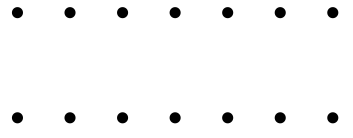
\includegraphics[width=.5\textwidth]{hw4_graphic1}
            \end{center}

            \begin{enumerate}[(a)]
                \item How many quadrilaterals are possible?

                ${7\choose 2}{7\choose 2} = 441$ quadrilaterals

                \item How many are squares?

                5 squares

                \item How many are rectangles?

                ${7\choose 2}$ rectangles

                \item How many are parallelograms?

                There are ${7\choose 2} + ({7\choose 2} - 1) + ({7\choose 2} - 3) + ({7\choose 2} - 6) + ({7\choose 2} - 10) + ({7\choose 2} - 15) = 91$ parallelograms.

                \item How many are trapezoids? (Here, as in calculus, a trapezoid is defined as a quadrilateral with at least one pair of parallel sides. In particular, parallelograms are trapezoids.)

${7\choose 2}{7\choose 2} - \left[ {7 \choose 2} + ({7 \choose 2}-1) + ({7 \choose 2} - 3) + ({7 \choose 2} - 6) + ({7 \choose 2} - 10) + ({7 \choose 2} - 15) \right]\text{.}$

                \item How many are trapezoids that are not parallelograms?



            \end{enumerate}

        %6
        \item How many triangles are there with vertices from the points shown below? Note, we are not allowing degenerate triangles - ones with all three vertices on the same line, but we do allow non-right triangles. Explain why your answer is correct.

            \begin{center}
            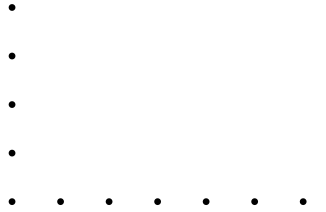
\includegraphics[width=.5\textwidth]{hw4_graphic2}
            \end{center}

            If you pick any three points, you can get a triangle, unless those three points are all on the x-axis or on the y-axis. There are other ways to start this as well, and any correct method should give the same answer. 120

        %12
        \setItemNumber{12}
        \item Consider sets $A$ and $B$ with $|A| = 10$ and $|B| = 17$.
            \begin{enumerate}[(a)]
                \item How many functions $f: A\rightarrow B$ are there?

                    $17^10$ functions. There are 17 choices for the image of each element in the domain.

                \item How many functions $f: A\rightarrow B$ are injective?

                    $P(17, 10)$ injective functions. There are 17 choices for image of the first element of the domain, then only 16 choices for the second, and so on.

            \end{enumerate}

    \end{enumerate}


	
	\paragraph{Problem 4} Counting Proofs\\

	Given what you've learned from chapter 1.4 about the difference between calculation and proofs, write up a proof or explanation for the following statement:\\

	\textbf{A full binary tree of depth $d$ has $2^{d-1}$ leaves.} \\

	(Recall that a full binary tree is a binary tree where every path is the same length, i.e. all the leaf nodes are at the same depth.)
	
		
\end{document}
	
